\section{Лекция 1. Обыкновенные дифференциальные уравнения}
\noeqref{eq:l1_ode_gen, eq:l1_ode_res, eq:l1_ode1_imp, eq:l1_ode1_exp}
\noeqref{eq:l1_ex_star, eq:l1_cauchy_eq, eq:l1_cauchy_ic}

\begin{flushright}
    07.09.26
\end{flushright}

\subsection{Основные понятия и определения}

\begin{definition}
    Уравнение вида
    \begin{equation} \label{eq:l1_ode_gen}
        F\left(x, y, y', \dots, y^{(n)}\right) = 0 \tag{1}
    \end{equation}
    называется \textdef{обыкновенным дифференциальным уравнением (ОДУ)}, где:
    \begin{itemize}
        \item $x$ — независимая переменная;
        \item $y = y(x)$ — неизвестная (искомая) функция;
        \item $n \in \N$ — \textdef{порядок уравнения} (наивысший порядок
        производной, входящей в уравнение).
    \end{itemize}
\end{definition}

\begin{example} ~
    \begin{align*}
        x y'' + x^2 y' + y &= 0, & n &= 2, \\
        x (y')^3 + 2y - 3 &= 0, & n &= 1.
    \end{align*}
\end{example}

\begin{definition}
    Уравнение вида
    \begin{equation} \label{eq:l1_ode_res}
        y^{(n)} = f\left(x, y, y', \dots, y^{(n-1)}\right) \tag{2}
    \end{equation}
    называется обыкновенным дифференциальным уравнением,
    \textdef{разрешённым относительно старшей производной}.
\end{definition}

\begin{example} ~
    \begin{align*}
        y'' &= y^3, \\
        y'' &= x y^3 - (y')^2.
    \end{align*}
\end{example}

\begin{remark}
    Нелинейное уравнение 2-го порядка вида $y'' = x^\sigma y^k$ в физике и
    астрофизике называется \textdef{уравнением Эмдена — Фаулера}.
\end{remark}

\subsection{Дифференциальные уравнения 1-го порядка}

В общем и разрешённом относительно производной видах дифференциальное
уравнение 1-го порядка записывается соответственно как:
\begin{align}
    F(x, y, y') &= 0, \tag{3} \label{eq:l1_ode1_imp} \\
    y' &= f(x, y). \tag{4} \label{eq:l1_ode1_exp}
\end{align}

\begin{designation}
    Здесь и далее через $C(I)$ обозначается множество всех функций,
    непрерывных на интервале $I \subset \R$, а через $C^n(I)$ (где
    $n \in \N \cup \{\infty\}$) — множество функций, имеющих на $I$
    непрерывные производные до порядка $n$ включительно.
\end{designation}

\begin{definition}
    \textdef{Решением дифференциального уравнения} порядка $n \ge 1$ на
    интервале $I \subset \R$ называется любая $n$ раз дифференцируемая на $I$
    функция $y = y(x)$, обращающая это уравнение в тождество при всех
    $x \in I$.
\end{definition}

\begin{example}
    Рассмотрим простейшее дифференциальное уравнение 1-го порядка:
    \begin{equation} \label{eq:l1_ex_star}
        y' = x \tag{5}
    \end{equation}
    Любая функция вида $y(x) = \dfrac{x^2}{2} + C$, где $C \in \R$, принадлежит
    классу $C^1(\R)$ и является решением уравнения \eqref{eq:l1_ex_star}.
\end{example}

\begin{definition}
    \textdef{Общее решение} — это семейство функций $y = \phi(x, C)$,
    зависящее от произвольной постоянной $C$, которое содержит все решения
    данного дифференциального уравнения (в рассматриваемой области) и только
    их.
\end{definition}

\begin{definition}
    \textdef{Частное решение} — любая конкретная функция $y = \phi(x, C_0)$,
    получаемая из общего решения при фиксированном значении постоянной
    $C = C_0$ (или обращающая уравнение в тождество).
\end{definition}

Для уравнения \eqref{eq:l1_ex_star} имеем:
\begin{itemize}
    \item Общее решение: $y = \dfrac{x^2}{2} + C, \quad C \in \R$.
    \item Частные решения: $y = \dfrac{x^2}{2}$ (при $C = 0$),
    $y = \dfrac{x^2}{2} + 1$ (при $C = 1$) и т. д.
\end{itemize}

Чтобы выделить конкретное частное решение из бесконечного семейства кривых,
задают дополнительное условие прохождения графика через фиксированную точку
$(x_0, y_0) \in \R^2$:
\[
    y(x_0) = y_0.
\]

\begin{definition}
    Задача нахождения решения дифференциального уравнения, удовлетворяющего
    заданному начальному условию:
    \begin{align}
        y' &= f(x, y), \tag{6} \label{eq:l1_cauchy_eq} \\
        y(x_0) &= y_0, \tag{7} \label{eq:l1_cauchy_ic}
    \end{align}
    называется \textdef{задачей Коши}.
\end{definition}

\begin{proof}[Решение задачи Коши для уравнения \eqref{eq:l1_ex_star}]~\\
    \begin{quote}
        Составим систему из общего решения уравнения \eqref{eq:l1_ex_star} и
        начального условия \eqref{eq:l1_cauchy_ic}:
        \[
            \begin{cases}
                y = \dfrac{x^2}{2} + C, \\
                y(x_0) = y_0.
            \end{cases}
        \]
        Подставим координаты начальной точки $(x_0, y_0)$ и выразим $C$:
        \[
            y_0 = \frac{x_0^2}{2} + C \implies C = y_0 - \frac{x_0^2}{2}.
        \]
        Подставляя найденную константу обратно, получаем искомое частное
        решение:
        \[
            y(x) = \frac{x^2}{2} + y_0 - \frac{x_0^2}{2}.
        \]
        В частности, для начального условия $y(1) = 2$ находим:
        \[
            2 = \frac{1}{2} + C \implies C = \frac{3}{2} \implies
            y(x) = \frac{x^2}{2} + \frac{3}{2}.
        \]
    \end{quote}
\end{proof}

\begin{figure}[H]
    \centering
    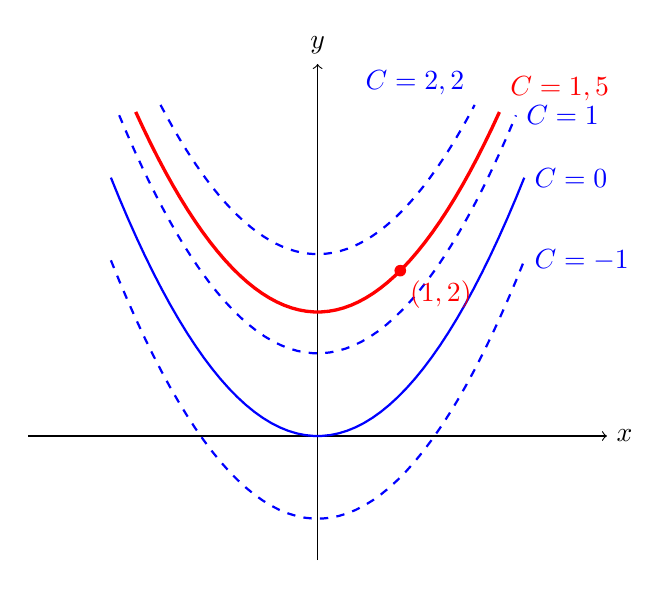
\begin{tikzpicture}[scale=1.05]
        % Оси координат
        \draw[->] (-3.5, 0) -- (3.5, 0) node[right] {$x$};
        \draw[->] (0, -1.5) -- (0, 4.5) node[above] {$y$};

        % Семейство парабол (общее решение)
        \draw[blue, thick, domain=-2.5:2.5, samples=50]
            plot (\x, {0.5*\x*\x}) node[right] {$C = 0$};
        \draw[blue, thick, dashed, domain=-2.4:2.4, samples=50]
            plot (\x, {0.5*\x*\x + 1}) node[right] {$C = 1$};
        \draw[blue, thick, dashed, domain=-1.9:1.9, samples=50]
            plot (\x, {0.5*\x*\x + 2.2}) node[above left] {$C = 2,2$};
        \draw[blue, thick, dashed, domain=-2.5:2.5, samples=50]
            plot (\x, {0.5*\x*\x - 1}) node[right] {$C = -1$};

        % Фиксированная точка и решение задачи Коши
        \draw[red, very thick, domain=-2.2:2.2, samples=50]
            plot (\x, {0.5*\x*\x + 1.5}) node[above right] {$C = 1,5$};
        \fill[red] (1, 2) circle (2pt) node[below right] {$(1, 2)$};
    \end{tikzpicture}
    \caption{Семейство интегральных кривых $y = x^2/2 + C$ и выделенное
    решение задачи Коши, проходящее через точку $(1, 2)$.}
\end{figure}

\begin{remark}
    В общем случае для произвольного уравнения вида \eqref{eq:l1_cauchy_eq}
    решение задачи Коши может оказаться неединственным. Условия существования
    и единственности будут строго сформулированы в Лекциях 2–4.
\end{remark}

\subsection{Геометрический смысл уравнения $y' = f(x, y)$}

В каждой точке $(x_0, y_0)$ из области определения $D \subset \R^2$ функции
$f(x, y)$ уравнение \eqref{eq:l1_ode1_exp} задаёт значение производной
$\left. y' \right|_{(x_0, y_0)} = f(x_0, y_0)$, то есть угловой коэффициент
$\tan \alpha = f(x_0, y_0)$ касательной к графику решения $y(x)$, проходящего
через эту точку.

\begin{definition}
    Совокупность точек плоскости $Oxy$ с привязанными к ним единичными
    отрезками, наклонёнными к оси $Ox$ под углом $\alpha = \arctan f(x, y)$,
    называется \textdef{полем направлений} дифференциального уравнения.
\end{definition}

\begin{definition}
    Гладкая кривая на плоскости $Oxy$, которая в каждой своей точке касается
    вектора поля направлений, называется \textdef{интегральной кривой}
    дифференциального уравнения.
\end{definition}

\begin{figure}[H]
    \centering
    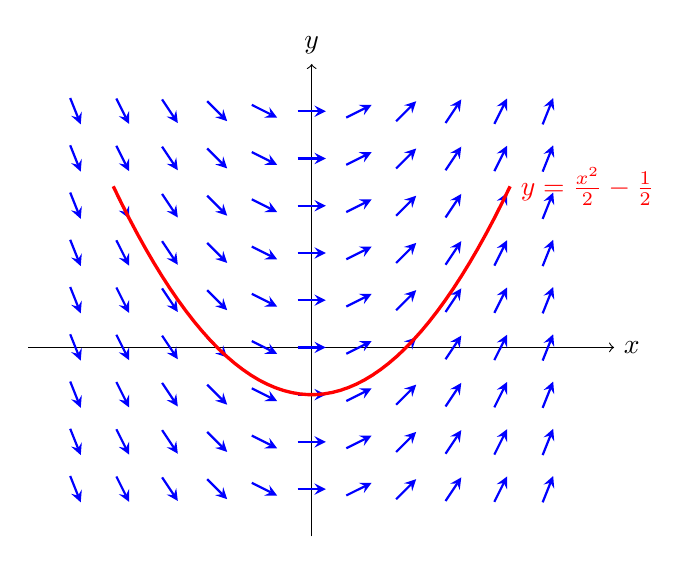
\begin{tikzpicture}[scale=1.2]
        % Оси координат
        \draw[->] (-3, 0) -- (3.2, 0) node[right] {$x$};
        \draw[->] (0, -2) -- (0, 3) node[above] {$y$};

        % Поле направлений y' = x
        \foreach \x in {-2.5, -2, ..., 2.5} {
            \foreach \y in {-1.5, -1, ..., 2.5} {
                \pgfmathsetmacro{\dx}{0.15 / sqrt(1 + \x*\x)}
                \pgfmathsetmacro{\dy}{0.15 * \x / sqrt(1 + \x*\x)}
                \draw[blue, thick, -stealth]
                    (\x - \dx, \y - \dy) -- (\x + \dx, \y + \dy);
            }
        }

        % Одна из интегральных кривых
        \draw[red, very thick, domain=-2.1:2.1, samples=50]
            plot (\x, {0.5*\x*\x - 0.5}) node[right] {$y = \frac{x^2}{2} - \frac{1}{2}$};
    \end{tikzpicture}
    \caption{Поле направлений и интегральная кривая для уравнения $y' = x$.}
\end{figure}

\begin{remark}
    Если интегральная кривая однозначно проектируется на ось $Ox$ (то есть
    каждому значению $x$ соответствует ровно одно значение $y$), то она
    является графиком некоторого решения $y = y(x)$. Однако интегральная
    кривая может иметь и точки с вертикальной касательной, в которых
    производная $y'_x$ обращается в бесконечность.
\end{remark}

\begin{definition}
    Геометрическое место точек плоскости, вдоль которого наклон поля
    направлений остаётся постоянным ($f(x, y) = k$, где $k = \text{const}$),
    называется \textdef{изоклиной}.
\end{definition}

\begin{figure}[H]
    \centering
    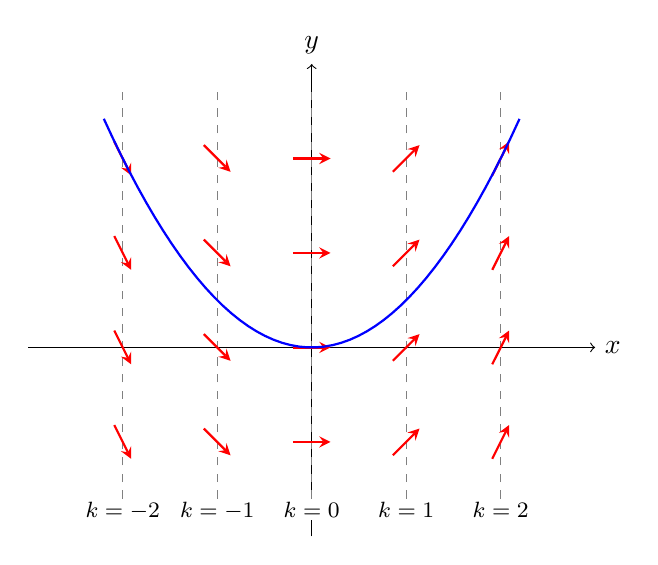
\begin{tikzpicture}[scale=1.2]
        % Оси координат
        \draw[->] (-3, 0) -- (3, 0) node[right] {$x$};
        \draw[->] (0, -2) -- (0, 3) node[above] {$y$};

        % Изоклины для y' = x (вертикальные прямые x = k)
        \foreach \k in {-2, -1, 0, 1, 2} {
            \draw[dashed, gray] (\k, -1.6) -- (\k, 2.7);
            \node[below, fill=white, inner sep=1pt]
                at (\k, -1.6) {\footnotesize $k = \k$};

            % Штрихи (направления) на изоклинах
            \foreach \y in {-1, 0, 1, 2} {
                \pgfmathsetmacro{\dx}{0.2 / sqrt(1 + \k*\k)}
                \pgfmathsetmacro{\dy}{0.2 * \k / sqrt(1 + \k*\k)}
                \draw[red, thick, -stealth]
                    (\k - \dx, \y - \dy) -- (\k + \dx, \y + \dy);
            }
        }

        % Пример построения кривой по штрихам изоклин
        \draw[blue, thick, domain=-2.2:2.2, samples=50]
            plot (\x, {0.5*\x*\x});
    \end{tikzpicture}
    \caption{Изоклины $x = k$, направления касательных и построенная по ним
    интегральная кривая для уравнения $y' = x$.}
\end{figure}

\subsubsection{Построение интегральных кривых методом изоклин}

\textbf{Алгоритм качественного построения фазового портрета:}
\begin{enumerate}
    \item Привести дифференциальное уравнение к разрешённому виду
    $y' = f(x, y)$.
    \item Выбрать характерный набор констант наклона $k \in \R$ (включая
    $k = 0$, что соответствует точкам экстремума решений).
    \item Для каждого фиксированного $k$ построить на плоскости $Oxy$ кривую
    изоклины $f(x, y) = k$.
    \item Вдоль каждой изоклины нанести короткие направляющие штрихи под
    углом $\alpha = \arctan k$ к положительному направлению оси $Ox$.
    \item Плавно соединить полученные направления интегральными кривыми,
    уточняя их выпуклость и асимптотику методами математического анализа.
\end{enumerate}